\section{Internet of Things}

\begin{frame}
\begin{center}
\Huge Internet of Things
\end{center}
\end{frame}

\begin{frame}
\frametitle{Overview}
\begin{itemize}
\item What is the Internet of Things?
\item Important aspects
\item Examples
\item Relevance to our project
\item Model-View-Controller
\item AJAX
\item SOAP
\end{itemize}
\end{frame}

\begin{frame}
\frametitle{What is the Internet of Things?}
\begin{itemize}
\item Concept describing interconnection of uniquely identifiable things in a problem domain
\item Real usage manifests as providing some service, permitting information flow and control over the problem domain
\item Prevalence - 30 billion devices connected to the IoT by 2020!
\end{itemize}
\end{frame}

\begin{frame}
\frametitle{Important aspects}
\begin{itemize}
\item Identification with IPv4 impractical
\item How to connect things
\item Low-cost \& low-power
\end{itemize}
\end{frame}

\begin{frame}
\frametitle{Examples}
\begin{itemize}
\item Smart house
\item Smart power grid
\end{itemize}
\end{frame}

\begin{frame}
\frametitle{Smart house}
\begin{center}
\begin{figure}
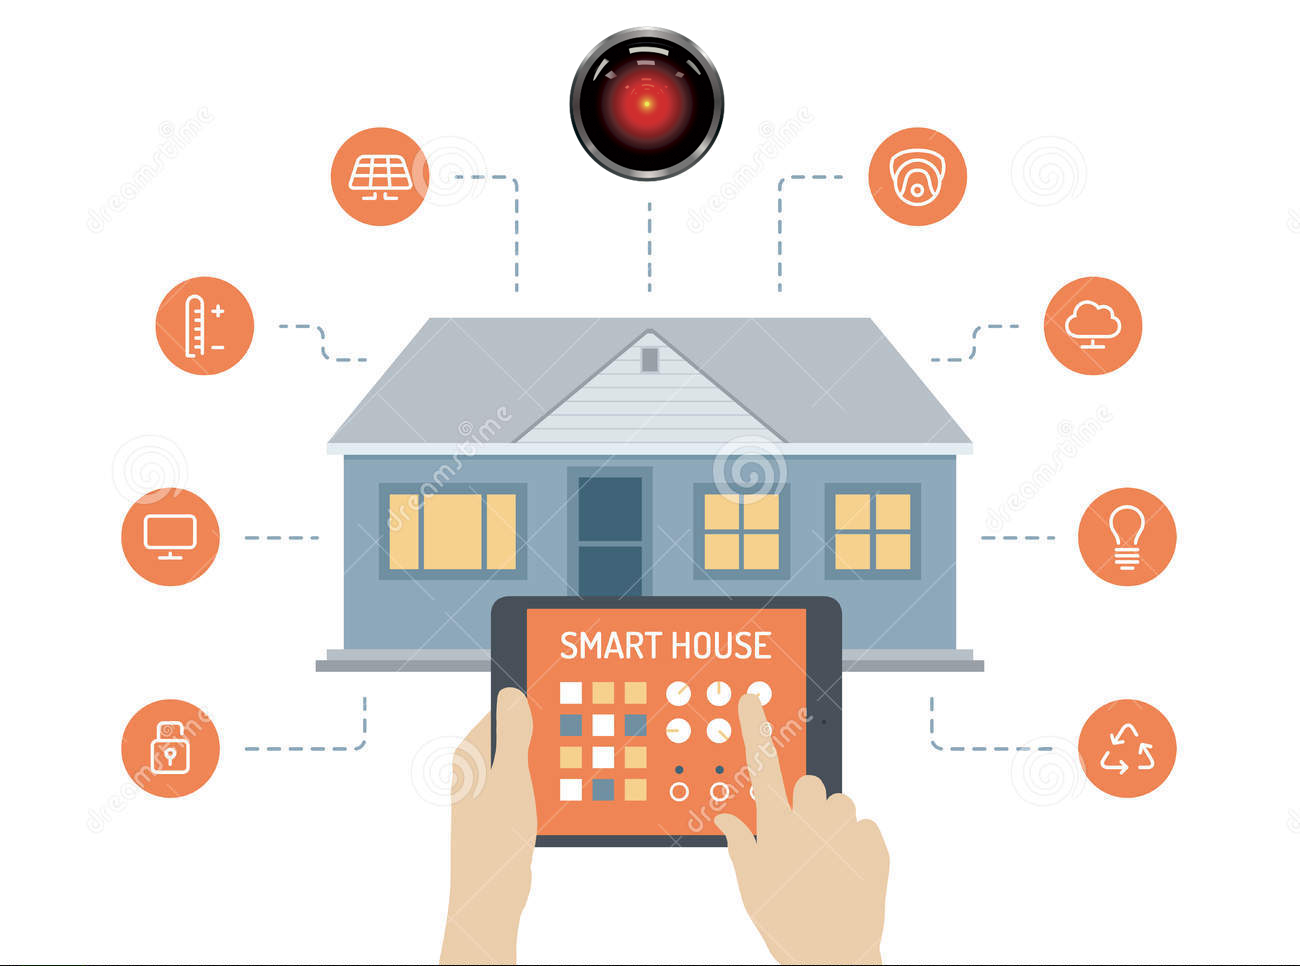
\includegraphics[scale=0.20]{smarthouse}
\caption{Source: dreamstime.com}
\end{figure}
\end{center}
\end{frame}

\begin{frame}
\frametitle{Smart power grid}
\begin{center}
\begin{figure}
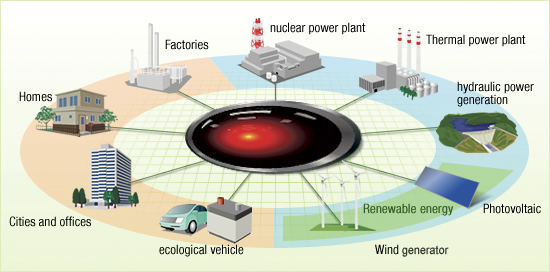
\includegraphics[scale=0.5]{smartenergygrid}
\caption{Source: hitachi.com}
\end{figure}
\end{center}
\end{frame}

\begin{frame}
\frametitle{Relevance to our project}
\begin{itemize}
\item General idea grounded in the Internet of Things
\item Multiple things interconnected and available to users
\item Important aspects: Status, location, providing user control over system
\end{itemize}
\end{frame}

\section{Technologies}
\begin{frame}
\begin{center}
\Huge Technologies
\end{center}

\end{frame}
\begin{frame}

\frametitle{Model-View-Controller}
\begin{itemize}
\item What is Model-View-Controller and how do we use it
\item Benefits: Clear code, organisation and architecture
\end{itemize}
\begin{figure}
\centering
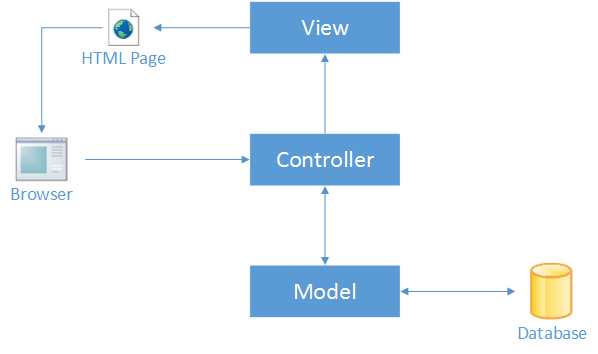
\includegraphics[scale=0.5]{MVC}
\end{figure}
\end{frame}

\begin{frame}
\frametitle{AJAX}
\begin{itemize}
\item Asynchronous updating, what is it and why should you use it?
\item Example: IMDb, giving a rating is asynchronous
\end{itemize}
\end{frame}

\begin{frame}
\frametitle{SOAP}
\begin{itemize}
\item Simple Object Access Protocol, what is it?
\item Why SOAP over other methods? Standard protocol, easy to use and sufficient
\end{itemize}
\end{frame}